\chapter{Déroulement du Stage}
\label{main}

% -=+=-
% RESUME
% -=+=-

\section{Information sur le sujet}

Pour pouvoir debuter le stage correctement, il était nécessaire de s'informer correctement sur le sujet traité et les sujets adjascents.
Il était aussi important de pouvoir se familiariser avec les usages des publication scientifique, de pouvoir s'entraîner a correctement
lire ce genre de publications.
C'est pourquoi on m'as proposer plusieurs articles à décortiquer, que j'ai résumé simplement, tout au long du stage.

\subsection{Format et Rendu}

Le format de résumé que j'ai choisi est ASCIIDOC, qui permet un formattage similaire à Markdown (avec un peu plus de possibilités), et une exportation facile en HTLM grâce à asciidoctor.

Les sources de ces documents sont hébergées sur une repository mise à ma disposition sur le groupe GitHub du PROGRESS:
\url{https://github.com/labri-progress/llm-study-zoo}

L'affichage Github n'éttant pas complet (n'affiche pas les documents importés, entre autres), j'ai décidé de rendre disponible un version rendue
\href{https://maxime-pico.emi.u-bordeaux.fr/stage-labri/llm-study-zoo/}{sur ma page CREMI}.


\subsection{Résumés}

Cette section passera rapidement sur les différents sujets présentés dans les articles que l'on m'a confié, ainsi que ce qui a pu etre tiré de l'article pour etre employé au cours du stage.
Pour des résumés plus détaillés, il est préférable d'aller voir \href{https://maxime-pico.emi.u-bordeaux.fr/stage-labri/llm-study-zoo/}{le rendu html sur ma pas CREMI}


\subsubsection{Empirical study on Code Completion Tools \cite{evalcodecompquality}}

Cet article présente une expérience de comparaison de performances entre
3 modèles de complétions sur un dataset de petites fonction avec leurs documentation.

Ce type d'experience m'as permi de voir le type d'expérimentation possible pour ce genre d'outils ainsi que
les types de mesures qui puissent être utilisées.


\subsubsection{Offline evaluation of Code Completion Tools \cite{llm-online-offline}}

Cet article présente une expérience de comparaison de performances entre
3 modèles de complétions, cette fois-ci open-sources, sur \href{https://github.com/VHellendoorn/Code-LMs#datasets}{un dataset multilangues}

Comme le précendent, il s'agit ici de voir la mise en placce de l'expérience et les metrics.


\subsubsection{Online evaluation of Code Completion Tools \cite{llm-online-offline}}

Cette section fait partie de l'article précendant, il s'agit de la deuxième partie de l'expérience.
Il s'agit ici d'évaluer d'un point de vue qualitatif et quantitatif les différents modèles "dans la nature",
c'est à dire directement en les testant auprès de développeurs pendant leurs sessions de travail.

On est ici sur un expérience plus proche que ce qui peut nous interesser pour notre sujet: une expérimentation avec directement sur des développeurs.


\subsubsection{Grounded Copilot: How Programmers Interact with Code-Generating Models \cite{grouded}}

Cette publication m'as été proposée car c'est une "grounded theory".
Ce type de publication cherche à faire emmerger des hypothèses à partir de données récolté sur un expérience.

Ici les chercheurs on mis en avant différents états pendant la phase de développement.
Il pourrait-être interressant de les faire resortir dans nos expérience, et d'integrer cette différenciation de phases dans l'analyse des données.


\subsubsection{CodeAid: A classroom deployment of an LLM-based programming assistant \cite{codeaid}}

Il s'agit ici d'une expérience mise en place sur une classe universitaire durant un semestre visant a observer les comportement des étudiants
face à un outils d'assistance à la programmation.
Cet article est très intéressant, il nous permet de voir le type d'expériences qui peut etre mener pour notre projet, ce qu'il est possible de mettre en place.


\subsubsection{Productivity Assessment of Neural Code Completion \cite{productivity-assess}}

Cet article est l'un des dernier que j'ai traité, le résumé n'est pas complet, cependant, il nous a renseigné sur la manière dont on peut
quantifier la productivité (ressentie) grâce au taux d'acceptation des complétions proposées par les extensions.

% -=+=-
% EXPLO
% -=+=-

\section{Exploration des outils a tester}
\label{explo}

Il existe de nombreux outils permettant la suggestion de code via des modèles prédictifs, il s'agit donc de trouver celui qui va convenir le mieux au type d'expériences que l'ont veut mener.

On a vu dans la séquence précedante quelques article qui utilisait justement ce genre d'outils, mais avec des approches différentes:

\begin{itemize}
  \item \textbf{En utilisant un model/une extension pré-éxistante} et en observant les comportements \cite{grouded}, ou en outillant l'IDE \cite{productivity-assess}.
  \item \textbf{En créant un outil autour d'un model distant} tel que CodeAID \cite{codeaid}, qui discute via des API pour suggerer completions, ou d'autre proxy comme \href{https://continue.dev}{continue.dev}.
  \item \textbf{En hébergeant soit-même un modèle}, soit sur un serveur \cite{llm-online-offline}, soit sur la machine du développeur.
\end{itemize}

Pour des contrainte de temps et de complexité de mise en place, nous somme résté sur la première option et avont utilisé GitHub Copilot, auquel j'ai accès gratuitement de part mon statut d'étudiant.
De plus, de nombreux autres outils nécessitaient beaucoup de performances à faire tourner, ou ne fonctionnaient pas du tout.

% -=+=-
% CODEGRITS
% -=+=-

\newpage
\section{Prise en main et modification de CodeGRITS}

CodeGRITS est un outils d'enregistement pour des sessions de développement sous IntelliJ IDEA (et IDE dérivés), Il m'a été proposé par mes encadrant comme un
piste potentielle pour pouvoir enregister les intéractions avec les models/extensions de completion de code assités par IA.

Comme dit précedement dans \ref{explo}, le model/extension sur lequel mon stage s'est concentré est GitHub Copilot, c'est l'outils autour duquel j'ai intrumenté CodeGRITS.

Le but ici était de chercher si est possible d'utiliser CodeGRITS avec GitHub Copilot pour récuperer des informations pendant la session de développement, tel que la suggestion d'un complétion et l'acceptation.

Tout les changements apportés à l'extensions sont publiés sur un fork de la repo sur mon compte GitHub personel: \url{https://github.com/Syudagye/CodeGRITS}


\subsection{Exploration}

Dans un permier temps, il a fallu explorer l'extension, voir ce qui était proposé par l'outil et ainsi voir ce qui allait être nécessaire à ajouter
pour arriver a quelque chose qui nous convienne dans le contexte d'un potentielle experience.


\subsubsection{Mise à jour}

La première étape était de faire foncionner l'extension CodeGRITS en soit.
Celle-ci étant faite pour les IDE IntelliJ antérieurs aux versions 2024 (voir figure \ref{codegrits-old-build-version}), il a fallu l'adapter
(c.f. commit \href{https://github.com/codegrits/CodeGRITS/commit/cdb10bcba529d050bfcb6c3693256f0e18450dad}{cdb10bc}).
En effet, afin d'eviter de chercher un moyens de downgrade mon installation d'intellij sur mon environement de travail (installé sous NixOS avec Flatpak),
j'ai préféré mettre à jour l'extension elle-même.
Même si celà aurais pû poser de potentiels problèmes de compatibilité, ça aurait été quelque chose d'intéressant à faire, et a proposer aux développeurs
de l'extensions pour améliorer leur outil.


\subsubsection{Données}

L'extension récupère des données sur la session de développement et les engeristre dans un dossier à la racine du projet ouvert dans l'IDE.
Il a fallu donc décortiquer la structure de ce dossier et des fichiers qui y sont contenus. Heureusement, ces données sont faite pour être facilement exploitables, la structure du dossier est donc très explicite:

\begin{itemize}
	\item Un dossier \lstinline{archives} contenant des sauvegardes des fichiers sources modifiés
	\item Un dossier \lstinline{screen_recording} contenant un fichier video de l'écran pendant la session
	\item Un fichier \lstinline{ide_tracking.xml} contenant différents événements émanant de l'éditeur pendant la session
\end{itemize}

Ce qui nous intéresse là dedans sont les données contenues dans les fichier xml, car c'est ici qu'il peut y avoir des évenements pertinants dans le contexte de Copilot.

Malheureusement, celà n'as pas été completement le cas: En effet, seul un événement relatif à l'insersion d'un complétion dans le texte source
(voir figure \ref{apply-inlay-action}) n'est enregisté.

\begin{figure}
	\centering
	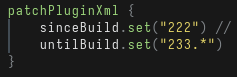
\includegraphics[width=7cm]{images/codegrits-wrong-version.png}
	\caption{Commande limittant les version utilisable d'IntelliJ}
	\label{codegrits-old-build-version}
\end{figure}

\begin{figure}
	\centering
	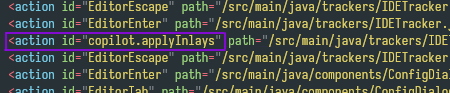
\includegraphics[width=10cm]{images/apply-inlay-action.png}
	\caption{Entrée du fichier \lstinline{ide_tracking.xml} référant à un évenement de complétion accéptée}
	\label{apply-inlay-action}
\end{figure}


\subsection{Modification}

Après avoir identifié les points manquants de l'extension CodeGRITS, il fallait maintenant trouver comment pallier à ce manque
en modifiant l'extension pour nos usages spécifiques.
À ce stade, il nous faut un moyens de tracker les moment ou l'extension Copilot viens suggerer du code au développeur, et que celui ci est visible
en grisé dans l'éditeur.

Plusieurs pistes on été envisagées, comme intercepter le traffic réseau entrant dans l'IDE, mais cela posait beaucoup de problème, nottament avec SSL.

Une approche beaucoup plus simple consistait à regarder les \emph{inlays} qui apparaissent dans l'éditeur,
c'est à dire les petits textes virtuels qui viennent donner des indications directement dans le viewport de l'éditeur de fichier,
comme par exemple le nom des paramêtre des fonctions, etc.

\subsubsection{Decompilation de Copilot}

GitHub Copilot n'étant pas du logiciel libre, il est impossible de regarder sont code de manière direct dur un depot publique, il faut donc trouver un autre moyens.
Heureusement, IntelliJ IDEA étant construit avec des technologies utilisant Java et la JVM, ses plugins aussi, il est donc possible de facilement décompiler l'extension afin de s'assurer de son fonctionnement.

\section{Analyse des données}

Lecture et structuration des données, création de graphs avec matplotlib, exploration de librairies plus intéractives (d3js, plotly)

\section{Soutenances de thèses (bonus)}

Vers la fin du mois de juin, j'ai pu assister a deux soutenances de thèses au sein du LaBRI.
